\section{The user interface}

Using the user stories and requirements introduced in earlier chapters, a new Autograder front-end has been designed. A lot of time was spend figuring out how the users tasks and workflows can be improved. Having discussed this with the client, Hein Meling, it was decided that extra time would be used on the layout of the four pages presented below.

\begin{description}
\item [Left panel] Used for "local" navigation. Navigate between student, teacher, settings etc. in an easy manner within the currently selected course. Mainly used to hide content that is not relevant at the current time (i.e settings page, score page).
\item [Middle panel] The most important content is placed in the middle. This is usually a table or list of students or roles.
\item [Right panel] This panel shows extended information about what is in the middle of the page. Actions in the middle panel triggers updates to the right panel.
\item [Course toggler] Placed above all the other panels, in the middle, it is used to toggle between active courses. All users will see this on the relevant pages. Designed to make switching between courses easier, it also removes the need to redirect to change courses.
\end{description}

\subsection{The homepage}
The homepage lists all the current courses for the logged in user. The courses shown depend on the roles of the user. All roles will be presented on the homepage. Courses the user can join are also listed here, to make the process of attending a new course easily accessible. Users can also request teaching permissions from the frontpage.

\begin{figure}[h!]
	 \centering
   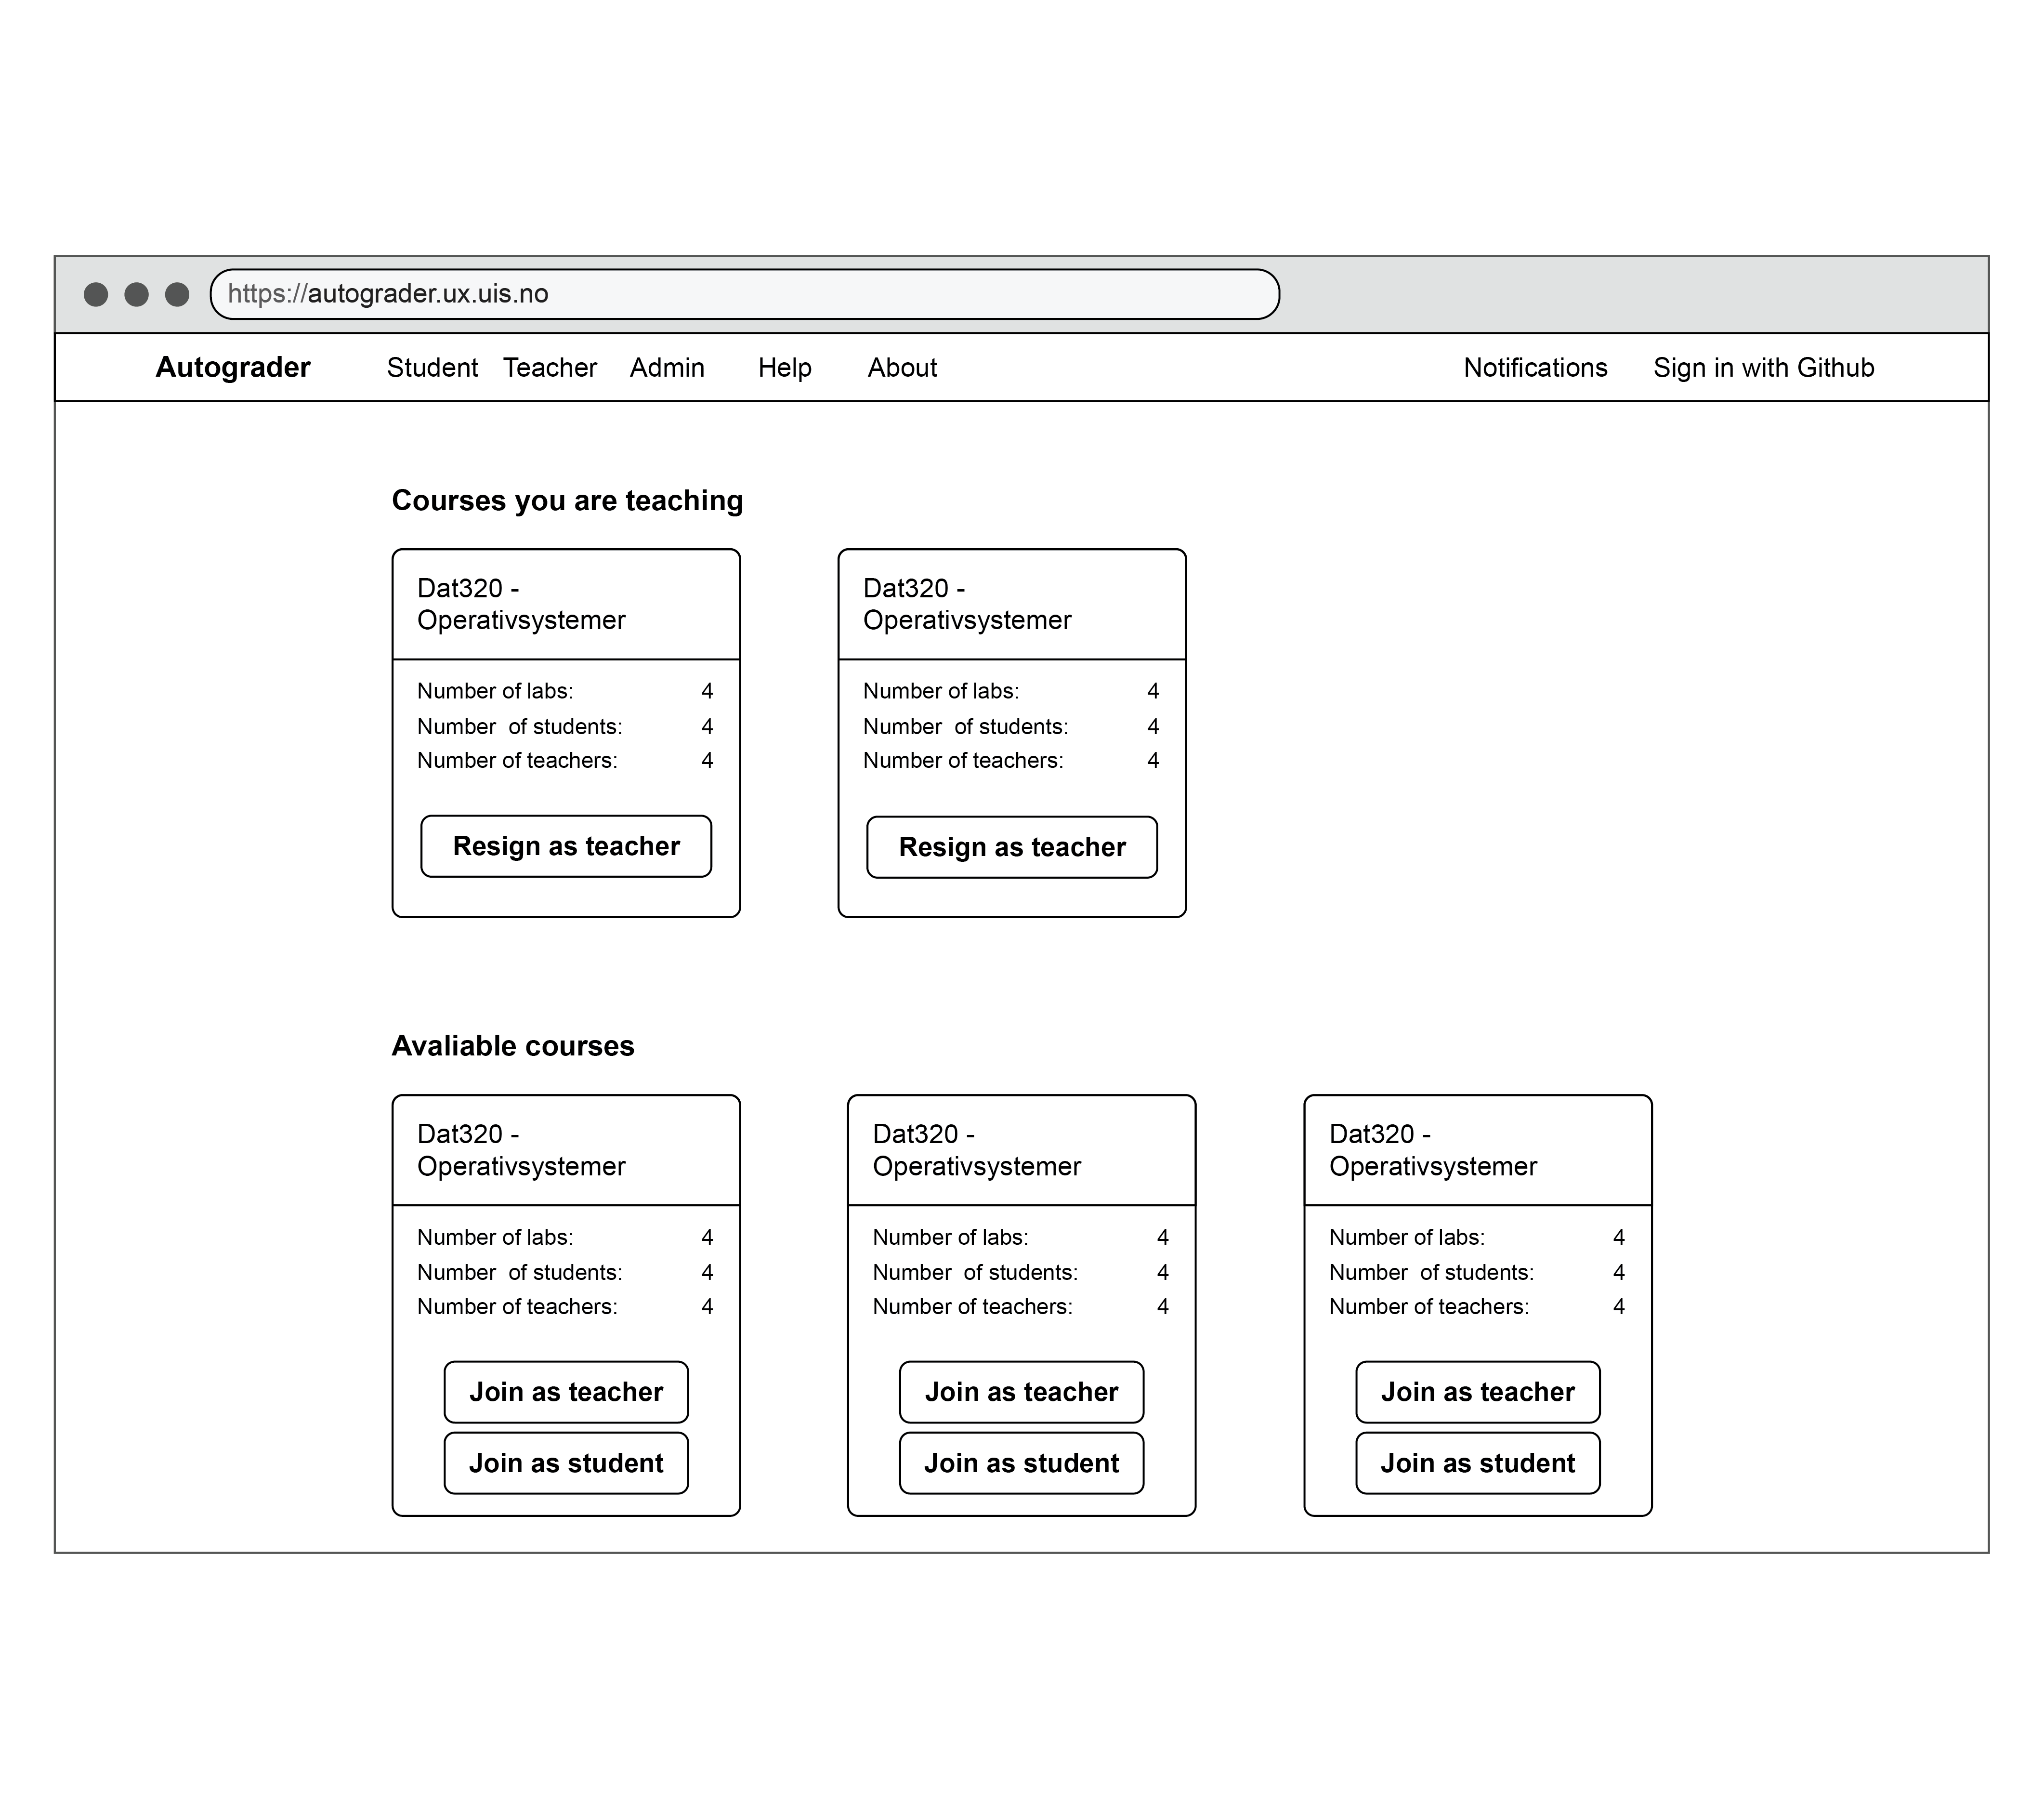
\includegraphics[width=1\textwidth]{homepage.png}
   \caption{The front page of the new Autograder}
   \label{fig:Wireframes for the new Autograder front-end}
\end{figure}

Figure \worry{figure ref above} shows the wireframe for the homepage of the new Autograder front-end. Each course has it's own card, with buttons for quick managment of user roles. Each card also shows some basic information from the course, such as number of labs, students and teachers. Clicking on the card, will redirect the user to the course clicked. As said, users can also view a list of all available courses as cards on the bottom of the page.

\subsection{The lab view}
The lab view has gone through several iterations, both in terms of design and layout. The original Autograder requires the teacher to visit each student's "page", where all the labs are listed for the currently selected student. The teacher grading the assignments has to go back end forth between the student page and the full list of students for every approval. Approving labs requires three redirects for every lab approved. Approving a class of 10 students requires 30 redirects, imagine a class of 50. The new Autograder front-end removes the need for page switching, by introducing the right side panel with lab view. Adding the right side "lab view panel" as seen in the wireframe on the right side, labs can be approved on the same page as the students are listed. A teacher can approve and view the lab results in the same window, for all students, removing the need to redirect the user.

\begin{figure}[h!]
	 \centering
   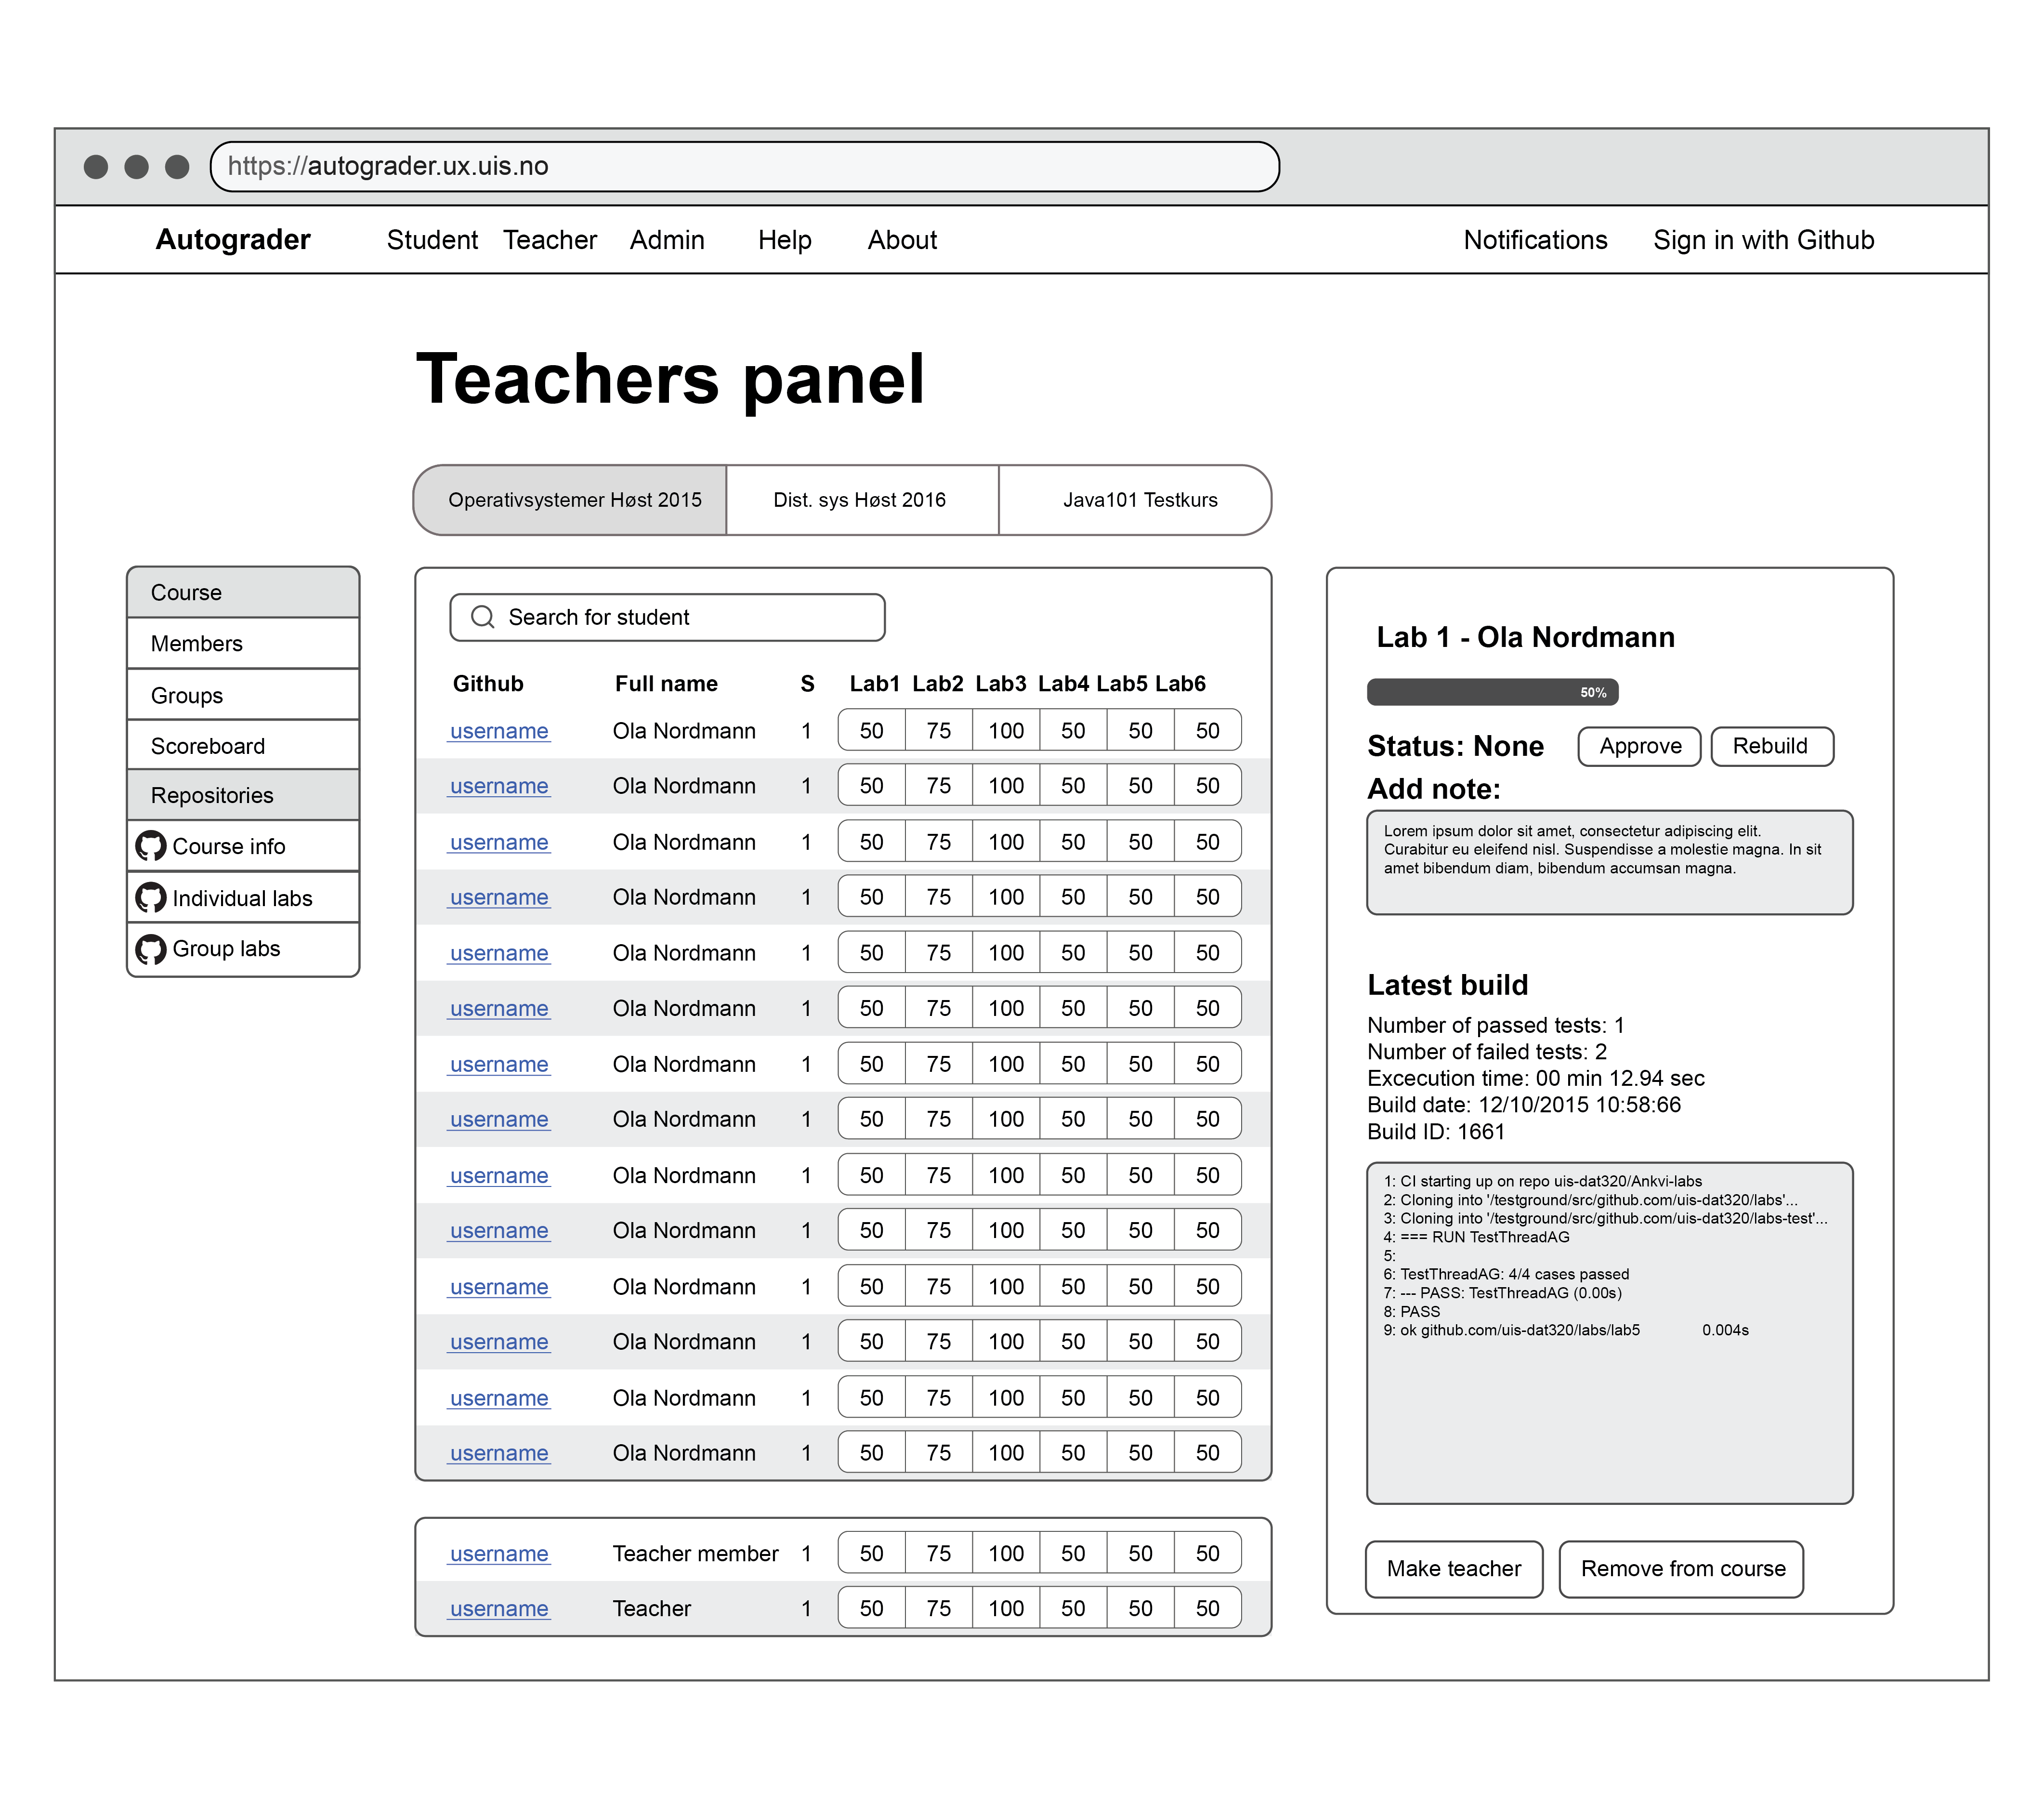
\includegraphics[width=1\textwidth]{labview.png}
   \caption{The view that teachers managing labs will have.}
   \label{fig:Wireframes for the new Autograder front-end}
\end{figure}

The teacher panel, as seen in figure \worry{Figure ref til den over}, is devided into four main parts. The left panel shows some navigation to other pages relevant for the teacher. The navigational bar over the middle panel, and under the header, is used to toggle between courses. This helps to remove unnecessary navigation between pages.

The middle panel shows all students in the currently selected course, as well as a search field. When a student is selected, the currently selected student will be updated, which will trigger an update in the right panel. The table form is used so that the number of labs can vary without effecting the layout of the page. When the number of labs exceed the amount of space assigned, the rest of the labs will be placed in a drop-down.

The right panel is designed to show the selected lab for a student, and triggers an update when the teacher clicks on another student. It is designed to show a summary of the currently selected lab, and implements functions to approve or rebuild the lab. A progress bar is also implemented, and will have colors to distinguish approved or failed labs. A build log is also implemented, and the results for the build process will be shown there. The teacher can also view an expanded view of the build log, which takes up the whole middle and right panel (not shown in the wireframe), to more efficiently view the log.

\subsection{Group manager}

Assignments that require groups can be created and managed in the group manager. The manager is designed to easily place students in groups. All the students in the course are listed in the middle panel. The right panel shows all groups and a button to create new groups. The teacher will select a group and add student in the selected group.

A requested feature from the client, Hein Meling, is that the teacher can use the group manager while the students are present in class. The teacher can go through the list of students, and place them in groups while the class i present, fast and simple. If the teacher chooses, it will also be possible to randomize groups. Another function of the group manager would be to implement a drag-and-drop, however, this is not implemented in the prototype. Figure \worry{REF TIL FIGUR} shows the wireframe for the group manager.

\begin{figure}[h!]
	 \centering
   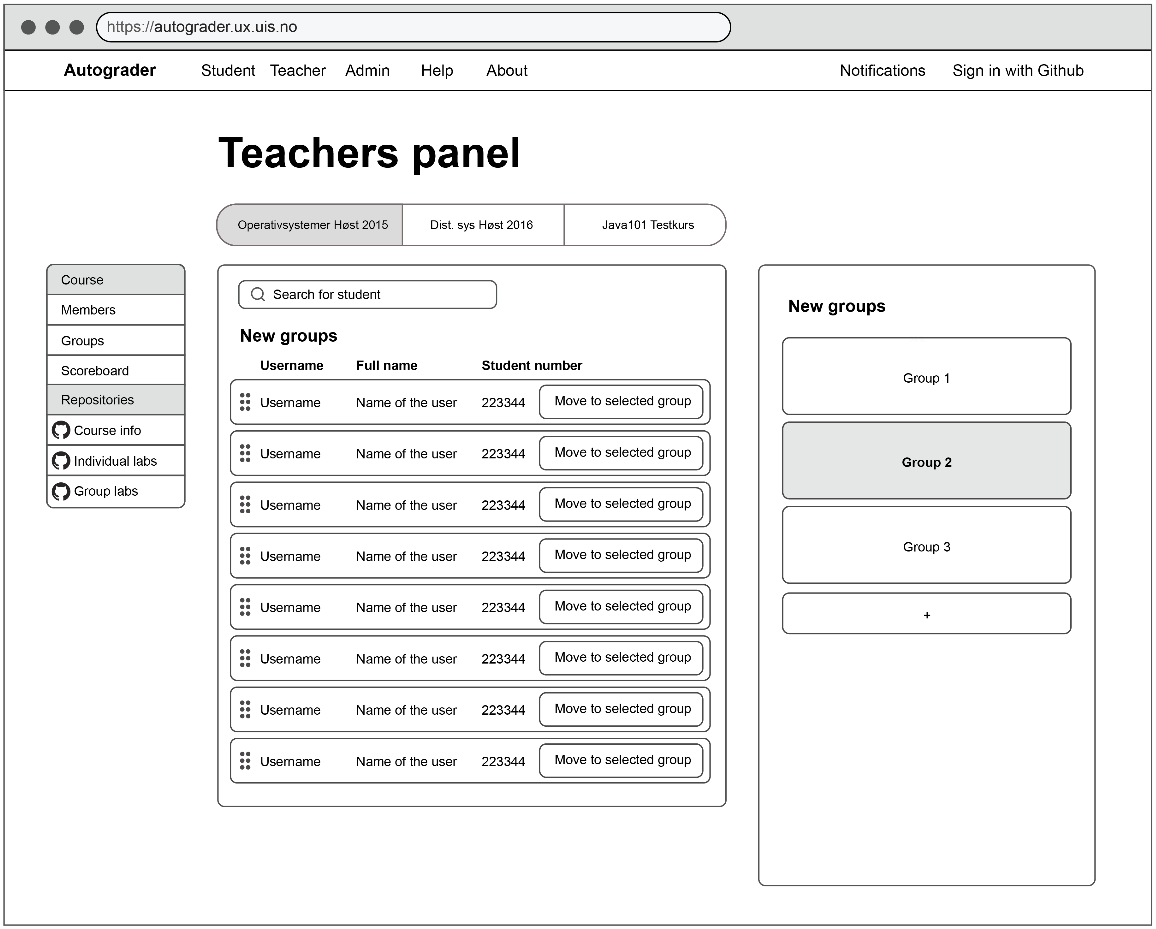
\includegraphics[width=1\textwidth]{groups.png}
   \caption{Group manager, seen as a wireframe.}
   \label{fig:Wireframes for the new Autograder front-end}
\end{figure}

\subsection{User manager}

The figure \worry{Ref til figure} shows the layout of the user manager. The left panel is used to toggle between different roles in the system. The system maintainer will use this view to change permissions for the Autograder system and remove users. Toggling between roles is made easy with the left side panel (student,teacher). The middle panel will show all the users with the selected role, i.e students and teachers.

\begin{figure}[h!]
	 \centering
   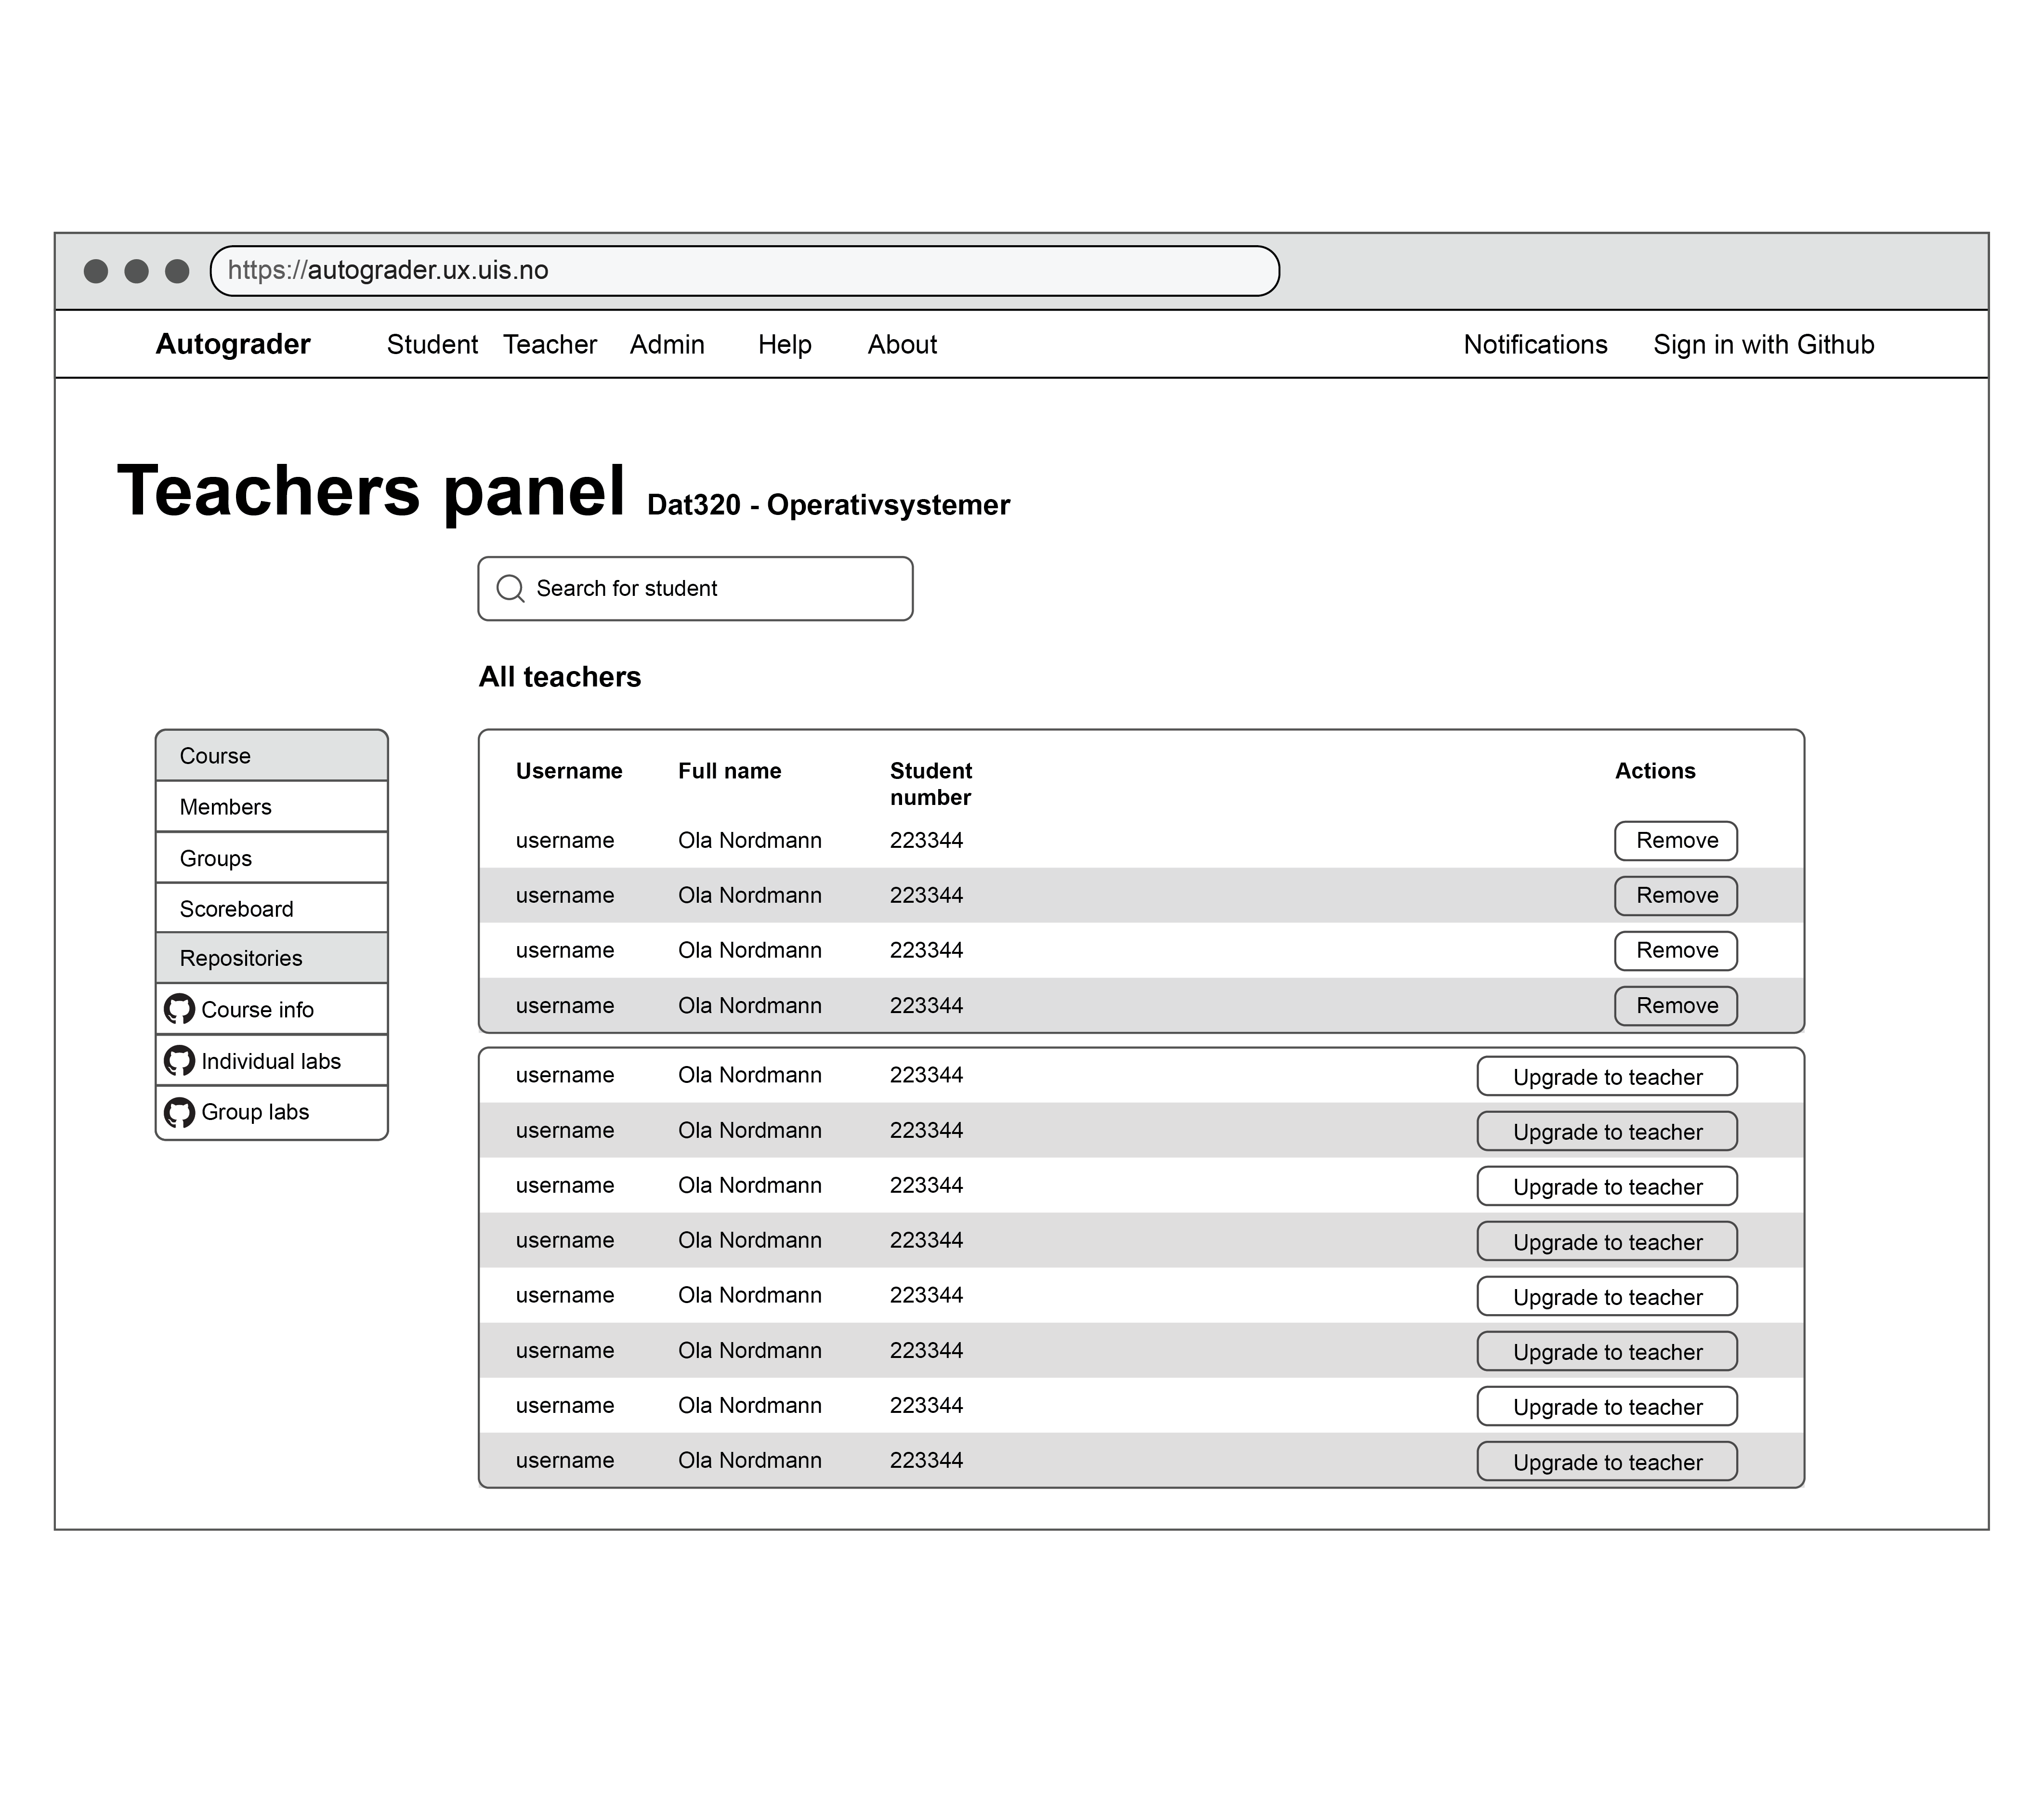
\includegraphics[width=1\textwidth]{roles.png}
   \caption{Page for managing roles in the system, specifically Admin, Teacher and Student}
   \label{fig:Wireframes for the new Autograder front-end}
\end{figure}






